\documentclass[12pt,a4paper]{scrreport}
\RequirePackage[2023/11/01]{latexrelease}
% Packages
% \usepackage[english]{babel}  
\usepackage[T1]{fontenc}    
\usepackage[utf8]{inputenc} 
\usepackage[left=3cm,right=2.5cm,top=2.5cm,bottom=2.5cm]{geometry}       
\usepackage{graphicx}       
\usepackage{hyperref}       
\usepackage[backend=biber]{biblatex}
\usepackage{easyReview}
\addbibresource{bibliography.bib} 
\usepackage{caption}
\usepackage{enumitem}
\usepackage{tcolorbox}
 \usepackage{booktabs}
\usepackage{tabularx}
 \usepackage{array}
   \usepackage{float} % Required for [H] placement
 % ---------- Layout ----------
\usepackage{setspace}
\onehalfspacing
% ---------- Math & Symbols ----------
\usepackage{amsmath,amssymb}
% ---------- Code Listings ----------
\usepackage{xcolor}
\usepackage{listings}
\lstset{%
basicstyle=\ttfamily\small,
columns=fullflexible,
showstringspaces=false,
breaklines=true,
frame=single,
framerule=0.2pt,
rulecolor=\color{black},
tabsize=2,
keepspaces=true
}
\captionsetup{labelfont=bf}
% Page Layout
% \geometry{left=3cm,right=2.5cm,top=2.5cm,bottom=2.5cm}
%Do not remove this file Y. Terchi
\newcommand{\cmt}[1]{\textcolor{red}{#1}}
\newcommand{\res}[1]{\textcolor{blue}{#1}}
\begin{document}

% Title Page
\begin{titlepage}
    \centering
    
\includegraphics[width=0.8\textwidth]{Figures/LOGO-UFAS1-2020.png} % University logo
    \\
    {\LARGE \textbf{Development of Modular Robotic Platforms}}\\[1cm]
    {\Large \textbf{for Development, Research and Education}}\\[2cm]
    \textbf{Presented by:} \textsc{Assil M. Ferahta}\\
    For the degree of \textbf{Masters} in \textbf{Embedded Systems Electronics}\\[1cm]
    \textbf{University:} Setif 1 Ferhat Abbas\\
    \textbf{Thesis Supervisor:} Dr. Younes Terchi\\
    \textbf{Date:} 2, 2025\\[2cm]

    \vfill
\end{titlepage}

% Front matter
\chapter*{Acknowledgments}

\chapter*{Abstract}
The development of modular robotic platforms has a set of problems with multiple possible solutions, therefore, defining a good concept to abide by is a good idea in order to realize such platforms and assure their flexibility, adaptability and uniqueness. In this thesis I will present my philosophies regarding the development of modular, upgradable and interchangeable components to form certain families of robotic platforms, as well as using them together to test different related concepts and emergent behavior between them.      
%more onto this later

%let's mention in this thesis the context of modularity, if modularity was a universe, our platforms are intended to reach different spaces AND different times unlike competition.

%let's also mention what we mean by space and time, space = dicipline or domain/field 
%time = level, target audience, learning ? developing ? children ? all levels of abstraction are tappable!

%add seciton about software support, talk about RTOS and code safety and such.
%talk about building on existing toolchains in literature such as Arduino UNO
%talk how we can expand by providing modules, upgrade kits and software support (Refer to sparkfun, digikey and such players).
%task it to maximize integration rates and domestic production.

% Table of Contents
\tableofcontents
\newpage

%Chapters
\chapter*{General Introduction}
Robotics has emerged as a pivotal technology in fields ranging from industrial automation and research to education and personal innovation. Despite rapid technological advances, a gap persists in providing accessible, versatile, and modular platforms that can cater to a diverse audience, ranging from researchers and students to hobbyists and ordinary users with minimal technical background. This thesis addresses this gap by introducing a set of modular robotic platforms; Bulky, Thegill, and $\mu$tomba, Dronegaze, alongside controllers like iLite and software tools for development and tinkering and interfacing which are designed with adaptability and ease of use in mind.

At the heart of this work is the idea of modularity as a means to bridge diverse domains from rigorous academic research and hands-on educational experimentation to hobbyist tinkering and everyday problem solving. Bulky is designed as a precision rover that integrates a flexible sensor-ready framework, exemplifying how a platform can evolve by accommodating custom modules. Thegill challenges conventional boundaries by operating seamlessly across terrestrial and aquatic environments, pushing the envelope on how modular components can harmonize mechanical adaptability with sophisticated control strategies. Meanwhile, $\mu$tomba distills robotics to its essentials, replacing rigid circuit boards with a breadboard setup to foster an environment of learning, rapid prototyping, and creative exploration.

Together, these platforms are not merely products with predefined applications; each platform embodies a distinct set of features and design philosophies while adhering to a common vision: to democratize robotics by offering modular and upgradable solutions that can be customized, extended, and integrated into various applications. They are conceptual testbeds that encourage users to tap on robotics via open design and abstraction. This thesis systematically explores the theoretical foundations of modular design, the practical integration of mechanical, software and electronic systems, and the experimental validation of these concepts. By doing so, it aims to demonstrate that embracing modularity and abstraction can transform robotics into a universally accessible and continually evolving field, empowering researchers, students, enthusiasts, and even everyday users to craft adaptive solutions in parallel of what is being developed in the industrial world.

This thesis documents the philosophy, problematic, design, implementation, and evaluation of these platforms, demonstrating how a modular approach can address a variety of challenges in robotics. It presents the theoretical foundations of modular design, details the system architecture, and evaluates the platforms through experimental testing. Ultimately, the work illustrates how such adaptable solutions can serve as universal products, empowering users to explore innovative applications in research, education, and beyond.

\section{Introduction to Modularity in Robotic Systems}
Modularity is a design philosophy that emphasizes constructing complex systems from smaller, self-contained components---commonly referred to as modules\footnote{Modules are discrete units of functionality that can be independently developed, tested, replaced, or upgraded.}. In the context of robotic platforms, this approach involves decomposing the system into discrete parts, each encapsulating specific functionalities such as sensing, actuation, communication, or processing, thereby simplifying design and troubleshooting.

At its core, modularity offers several significant benefits:

\begin{itemize}
  \item \textbf{Reusability}\footnote{Reusability refers to the ability to use developed modules in various configurations or projects, reducing overall development time and costs.}: Successfully developed and tested modules can be reused across different configurations or projects.
  \item \textbf{Flexibility}\footnote{Flexibility is the capacity to interchange or reconfigure modules to adapt to new requirements or experimental setups.}: Standardized interfaces\footnote{Interfaces are predefined methods for communication between modules, ensuring compatibility and ease of integration.} and communication protocols enable modules to be interchanged or reconfigured, a feature particularly valuable in rapid prototyping and iterative design.
  \item \textbf{Scalability}\footnote{Scalability describes the ease of integrating additional modules into an existing system as project requirements evolve.}: New modules can be integrated without necessitating a complete redesign, making it straightforward to expand functionality or incorporate emerging technologies.
  \item \textbf{Ease of Maintenance}\footnote{Ease of Maintenance refers to the capacity to replace or upgrade individual modules independently, thereby minimizing disruptions to the overall system.}: When a single module fails or becomes outdated, it can be replaced or upgraded without affecting the entire system.
\end{itemize}

In educational environments, modular robotic platforms serve as excellent teaching tools. They allow students to visualize and understand the intricate relationships between individual system components and the overall architecture. By experimenting with different module combinations, learners gain practical insights into system integration, problem-solving, and the inherent trade-offs in design decisions.

From a development perspective, modularity supports a more agile workflow. It enables parallel development, where different teams or individuals work simultaneously on separate modules. Upon integration, the overall system benefits from collective innovations, ensuring a robust and versatile platform. This design strategy also opens avenues for further innovation, as new modules can be developed to enhance system capabilities without overhauling the existing architecture.

Ultimately, adopting a modular approach in robotic platforms aligns perfectly with the goals of advancing research, fostering educational experiences, and enabling rapid prototyping. By leveraging the principles of modularity, developers can create adaptable and cost-effective platforms that meet the dynamic challenges of modern robotics.

\section{Notion of platforms}
Platforms can be considered a workspace that provides mechanical, electronic, software as well as energetic and power support for a project be it experimental or practical, but at the heart of this concept is "Abstraction", you don't need to understand how semiconductor or hardware works to work with an arduino for an instance, all you need is to be familiar with algorithms and programming; high level programming or even human language in our times of AI, no assembly or machine code anymore, but if you need to or want to go that low, it's still possible for you to do so, the arduino platform allows for all therefore:\\

\textbf{Definition.} A \emph{platform} is a deliberately stable core together with explicit contracts that enable independent parties to create, combine, and evolve extensions and applications over time without modifying the core.

\subsection{Platform vs. Product, Toolkit, Framework, Ecosystem}
% (Insert the comparison table here)

\subsection{Modular Robotic Platforms (MRP)}
An MRP exposes mechanical, electrical, and software contracts for safe composition of actuators, sensors, power, and behaviors.\\
"ASCE" platforms; what this thesis is about, follows an analogy: "if modularity is a universe, then our platforms allow freedom in both \textbf{space} and \textbf{time}"

\subsubsection{Space-Time Modularity}
Space = discipline (mechanical, electronics, software, logic/UX). 
Time = user maturity (consumer, learner, researcher, professional).

\subsection{The ASCE Platform Family}
% Formal tuple, shared philosophy, layers

\subsection{Minimum Viable Platform (MVPf)}
% 4 criteria list

\subsection{Axioms and Criteria}
% A1--A5 and testable criteria

\subsection{Platform Layers for Embedded Robotics}
% 8 layers list

\subsection{Contract Template}
% Per-interface template (IMU, ESC, Radio, etc.)

\subsection{Why ASCE is Different}
% Matrix argument and thesis claim



%ASCE Platforms is intedned to be a very modular platform that allows the users to customize the robots according to applications, this is by providing components at request.

%Such an approach would open the door to more potential ideas such as an interface to customize custom orders of such modular units to suite different professionl/industrial/developmental applications the user might require. it would also optimize the price of unit which may boost its commercial aspect.

%Initial ideas would only ivovle tires, custom prints on them or custom fins and sizes, even custom mecanuum wheels for different environments.







\chapter{Defining Platforms}\label{chap\:defining-platforms}
\section{Platform: Working Definition}\label{sec\:platform-definition}
A \emph{platform} is a deliberately stable core together with explicit contracts that enable independent parties to create, combine, and evolve extensions and applications over time without modifying the core.

Formally, we define a platform as the 5-tuple
\begin{equation}
\mathcal{P} = \langle \mathcal{C},; \Gamma,; \mathcal{E},; \mathcal{T},; \mathcal{G} \rangle,
\end{equation}
where $\mathcal{C}$ is the core, $\Gamma$ are the contracts (interfaces and guarantees), $\mathcal{E}$ are extensions, $\mathcal{T}$ are the tools, and $\mathcal{G}$ is governance.\\

These notions are commonly used in software design and computer science but we can apply the same philosophies behind them in our field of interest; robotics. 

\section{Origin of context}

The notion of a \emph{stable core with explicit contracts} emerges from three converging streams. First, modular design and information hiding established that software should be decomposed so that each module encapsulates design decisions behind stable interfaces, allowing implementations to vary without ripple effects \cite{parnas1972}. Second, \emph{Design by Contract} made those interface expectations explicit as preconditions, postconditions, and invariants, turning ``interfaces'' into formal \emph{contracts} between components \cite{meyer1992}. 

As software systems turned into industry platforms, researchers described architectures with a \emph{core} and a \emph{periphery of complements}, where the core's stability and the clarity of its interfaces enable independent evolution of complements. This core-complement view connects technical modularity to economic ecosystems and governance, giving a unified lens for platform design \cite{baldwin2009platforms}. 

In practice, the software-architecture community operationalized the idea through patterns such as the Hexagonal (Ports \& Adapters) Architecture: keep application logic independent of technology details, expose \emph{ports} as stable contracts, and attach \emph{adapters} for specific UIs, devices, or protocols. This preserves the core while enabling rapid replacement or addition of peripherals \cite{cockburn2005hexagonal}. 

Management and IS scholarship then integrated architecture with strategy and governance: how a platform owner maintains core stability, versioning, and compatibility while orchestrating third-party innovation. This literature articulates how interface design, API policies, and deprecation rules shape ecosystem health, providing the governance scaffolding that complements the technical contracts \cite{gawer2002platformleadership,tiwana2014platformecosystems}. 

Taken together, these threads justify the dissertation's framing: a platform is a deliberately stable core with explicit, versioned contracts that empower independent parties to create and evolve extensions over time, without modifying that core or building on top of it. This "core" may be rigid and not as flexible outside intended use cases, but we can add that missing dimension by making it "Modular"; the core is merely a solid kernel that allows for a huge variety of stock or third party modules (or adapters in the sense of hexagonal architecture) to plug in, letting the users shape it as they please (Spacetime liberty!).

\subsection{Platform vs. Product, Toolkit, Framework, Ecosystem}\label{subsec:platform-comparison}
The magic behind \textbf{\textit{ASCE}} platforms is that aside from being platforms, they may also behave as products, toolkits frameworks, and an ecosystem (Since modularity and hexagonal architecture philosophies allow for cross platform and emergent behavior).
\begin{table}[h]
\centering
\caption{Platform vs. related constructs}
\renewcommand{\arraystretch}{1.15}
\begin{tabularx}{\textwidth}{lXXXX}
\toprule
\textbf{Construct} & \textbf{Core intent} & \textbf{Who extends it?} & \textbf{Interface stability} & \textbf{Typical deliverables} \\
\midrule
Product   & Solve a specific use case             & Vendor             & n/a           & Device/app with fixed features \\
Toolkit   & Provide parts to assemble             & End user           & Low--Medium   & Components, examples \\
Framework & Invert control; fill hooks            & Developer          & Medium--High  & Base code + callbacks \\
Ecosystem & Community of complements              & Many parties       & Mixed         & Marketplaces, standards \\
\textbf{Platform} & \textbf{Stable core + contracts for many products} & \textbf{First\&third parties} & \textbf{High (versioned)} & \textbf{Core, interfaces, SDKs, docs, governance} \\
\bottomrule
\end{tabularx}
\end{table}

\section{Modular Robotic Platforms (MRP)}\label{sec:mrp}
A \emph{Modular Robotic Platform} (MRP) exposes mechanical, electrical, and software contracts for safe composition of actuators, sensors, power, and behaviors so that a wide range of robots can be built, upgraded, and repurposed without modifying the core.

\subsection{Space-Time Modularity}\label{subsec:space-time}
Space is \emph{discipline} (mechanical, electronics, software, logic/UX). Time is \emph{user maturity} (consumer, learner, researcher, professional). A high-quality MRP provides variation points across space and growth paths across time.

\begin{table}[H]
\centering
\caption{ASCE Space--Time matrix of modularity}
\renewcommand{\arraystretch}{1.2}
\begin{tabularx}{\textwidth}{lXXXX}
\toprule
\textbf{Time $\downarrow$ / Space $\rightarrow$} & \textbf{Mechanical} & \textbf{Electronics} & \textbf{Software} & \textbf{Logic \& UX} \\
\midrule
Consumer & Prebuilt mounts; safe geometry & Pre-wired modules & App presets & One-click modes, arming rules \\
Learner & Parametric parts & Labeled harnesses; rails & Config files; examples & Guided labs, wizards \\
Researcher/Dev & Custom frames; CoG guidance & Swappable drivers; EMI budget & Ports/adapters; SDK & Tests, CI, telemetry \\
Professional & Optimized rigs; stiffness specs & Power tiers; fusing; connectors & RT guarantees; schedulers & Toolchains, HIL, certification hooks \\
\bottomrule
\end{tabularx}
\end{table}

\section{Minimum Viable Platform (MVPf)}\label{sec:mvpf}
A \emph{Minimum Viable Platform} requires: (1) a stable, versioned contract with at least one extension point per relevant layer; (2) two distinct realizations exercising the contracts; (3) tooling to build/test/document extensions; and (4) governance for compatibility and deprecation.

\begin{table}[h]
\centering
\caption{MVPf checklist (evidence at submission time)}
\renewcommand{\arraystretch}{1.2}
\begin{tabularx}{\textwidth}{lX}
\toprule
\textbf{Criterion} & \textbf{Evidence artifact} \\
\midrule
Stable contract(s) & Interface spec (versioned), timing/error semantics, unit tests \\
Two realizations & e.g., Drone + Line-follower reusing core; alternate IMU/ESC drivers \\
Tooling & Templates, CI, documentation, simulator/HIL scripts \\
Governance & SemVer policy, compatibility matrix, deprecation schedule \\
\bottomrule
\end{tabularx}
\end{table}

\section{ASCE Contracts (Selected)}\label{sec:contracts}
This section provides concise, testable contract specifications for three key ports. Each contract includes functional semantics, timing, error model, and compliance tests. Versions use semantic versioning (e.g., \texttt{imu.v2}).

\subsection{IMU Port (\texttt{imu.v2})}\label{subsec:imu-contract}
\begin{description}
\item[Identifier \& Version] \texttt{imu.v2}.
\item[Functional Semantics] Provide linear acceleration $(a\_x,a\_y,a\_z)$ in $\mathrm{m/s^2}$ and angular velocity $(\omega\_x,\omega\_y,\omega\_z)$ in $\mathrm{rad/s}$; right-handed body frame; timestamps in microseconds since boot.
\item[Sampling] Required supported rates: {100, 200, 400} Hz; default 200 Hz. Report actual rate via \texttt{sampleRateHz()}.
\item[Timing Contract] End-to-end latency (sensor read $\rightarrow$ consumer) $< 2$ ms (typ.), jitter $< 500$ $\mu$s (95th percentile) at 200 Hz.
\item[Calibration] Bias/scale persisted via Store port; soft-iron/hard-iron optional; expose \texttt{setCalibration()} and \texttt{getCalibration()}.
\item[Error Model] Health states: \texttt{OK}, \texttt{DEGRADED} (auto-retrying), \texttt{FAILED} (requires reinit); provide error codes and backoff policy.
\item[Power/EMI] 3.3V logic; I\textsuperscript{2}C or SPI; max I\textsuperscript{2}C clock 400 kHz; bus hang recovery via clock stretching up to 9 pulses.
\item[Security/Integrity] Optional CRC in SPI; sequence counters for drop detection in DMA pipelines.
\item[Compliance Tests] (i) rate conformance; (ii) unit/axis sign tests; (iii) jitter histogram under CPU load; (iv) power brownout recovery; (v) hot-swap detection (if bus supports it).
\end{description}

\subsection{ESC Port (\texttt{esc.v1})}\label{subsec:esc-contract}
\begin{description}
\item[Identifier \& Version] \texttt{esc.v1}.
\item[Functional Semantics] Command normalized throttle $u\in[0,1]$; monotonic mapping to PWM or DSHOT. Provide \texttt{arm()}, \texttt{disarm()}, \texttt{write(u)}, \texttt{stop()}.
\item[Timing Contract] Update at 400 Hz (min). Command-to-output latency $<1$ ms typ.; report \texttt{lastWriteTime()}.
\item[Safety] Disarmed default; loss-of-signal watchdog $<50$ ms; min/max clamps; ramp-rate limits configurable.
\item[Error Model] \texttt{OK}, \texttt{TIMEOUT}, \texttt{BUS\_ERROR}, \texttt{OVERCURRENT} (if telemetried). Failsafe maps to \texttt{stop()}.
\item[Electrical] 3.3V PWM or digital protocol (e.g., DSHOT600); shared ground; specify rise/fall constraints for LEDC or timer units.
\item[Compliance Tests] (i) monotonicity sweep; (ii) timing scope traces; (iii) watchdog trip; (iv) arming sequence; (v) ramp-rate bound check.
\end{description}

\subsection{Radio Port (\texttt{radio.v1})}\label{subsec:radio-contract}
\begin{description}
\item[Identifier \& Version] \texttt{radio.v1}.
\item[Functional Semantics] Bidirectional datagrams with topics (e.g., \texttt{rc/*}, \texttt{telemetry/*}). Provide \texttt{publish(topic, payload)} and \texttt{subscribe(topic, handler)}.
\item[Timing Contract] Control path latency $<20$ ms one-way (95th percentile). Provide \texttt{rssi()} and link \texttt{quality()}.
\item[Error Model] Retries with exponential backoff; duplicate filtering via sequence numbers. Health: \texttt{OK}, \texttt{DEGRADED}, \texttt{DISCONNECTED}.
\item[Security] Optional pairing with nonce; packet authentication (HMAC) optional but recommended for professional tier.
\item[Compliance Tests] (i) range vs. latency curves; (ii) packet loss under interference; (iii) reconnect times; (iv) topic throughput fairness.
\end{description}

\section{Proof by Substitution: Swapping IMUs in Drongaz}\label{sec:proof-substitution-imu}
This section demonstrates that ASCE's ports \& adapters architecture allows replacing one IMU with another without changing the core (controllers, estimator, mixer, or telemetry schema).

\subsection{Port Interface (stable)}
\noindent\textbf{C++ Interface (header):}
\begin{lstlisting}[language=C++]
// Port: Imu (imu.v2)
struct ImuSample {
uint64\_t t\_us; // timestamp (us since boot)
float ax, ay, az;   // m/s^2
float gx, gy, gz;   // rad/s
};

enum class Health { OK, DEGRADED, FAILED };

class Imu {
public:
virtual \~Imu() {}
virtual bool begin() = 0;
virtual bool read(ImuSample& out) = 0; // non-blocking; returns false if no new sample
virtual float sampleRateHz() const = 0;
virtual Health health() const = 0;
};
\end{lstlisting}

\subsection{Two Adapters (variable)}
\noindent\textbf{Adapter A:} \texttt{Mpu6050Imu} implements \texttt{Imu} over I\textsuperscript{2}C.\\
\textbf{Adapter B:} \texttt{Icm20948Imu} implements \texttt{Imu} over SPI.

\begin{lstlisting}[language=C++]
class Mpu6050Imu : public Imu { /\* ... */ };
class Icm20948Imu : public Imu { /* ... \*/ };
\end{lstlisting}

\subsection{Dependency Injection into the Core}
The estimator depends only on the \texttt{Imu} port.
\begin{lstlisting}[language=C++]
class Estimator {
Imu& imu;
public:
explicit Estimator(Imu& ref) : imu(ref) {}
void tick() {
ImuSample s; if (imu.read(s)) { /\* predict-update using s \*/ }
}
};
\end{lstlisting}

\subsection{Build-Time Swap (no core edits)}
\begin{lstlisting}[language=C++]
// main.cpp (composition root)
\#ifdef USE\_ICM20948
static Icm20948Imu imu;
\#else
static Mpu6050Imu imu;
\#endif
static Estimator estimator(imu);
\end{lstlisting}

\subsection{Run-Time Swap via Factory (still no core edits)}
\begin{lstlisting}[language=C++]
// config.json (deployed via Store port)
// { "imu": { "driver": "icm20948", "rate\_hz": 400 } }

std::unique\_ptr<Imu> makeImu(const Config& cfg) {
if (cfg.imu.driver == "icm20948") return std::make\_unique<Icm20948Imu>(cfg);
if (cfg.imu.driver == "mpu6050")  return std::make\_unique<Mpu6050Imu>(cfg);
return nullptr; // TODO: handle error
}
\end{lstlisting}

\subsection{Invariants Preserved}
\begin{itemize}
\item Telemetry schema (units, axes, timestamps) unchanged (consumer code unaffected).
\item Controllers/mixer unaffected; only \texttt{Imu} adapter swapped.
\item RTOS task graph unchanged; timing contract verified against \texttt{imu.v2} tests.
\item No edits to core files (e.g., \texttt{FlightCore}, \texttt{Controllers}, \texttt{Mixer}, \texttt{Telemetry}).
\end{itemize}

\section{Contract Template (for New Ports)}\label{sec:contract-template}
Use the following template when specifying additional ports (e.g., \texttt{clock.v1}, \texttt{telemetry.v1}, \texttt{store.v1}).

\begin{enumerate}
\item \textbf{Identifier \& Version}: \texttt{<name>.v<major>}.
\item \textbf{Functional Semantics}: Inputs/outputs, coordinate frames, units, lifecycle.
\item \textbf{Timing Contract}: Rates, latency/jitter bounds, concurrency model, buffering.
\item \textbf{Error Model}: Health states, error categories, retry/backoff, degradation behavior.
\item \textbf{Safety}: Failsafe states, watchdogs, arming/disarming, clamping.
\item \textbf{Electrical/Mechanical (if applicable)}: Voltage/current, connectors, mounting patterns.
\item \textbf{Security/Integrity}: Auth, sequence numbers, CRCs, tamper evidence.
\item \textbf{Compliance Tests}: Automated checks, HIL procedures, acceptance thresholds.
\item \textbf{Deprecation Policy}: Compatibility window and migration notes.
\end{enumerate}


\chapter{Foundational Concepts in Robotics, Kinematics, and Interdisciplinary Integration}
\label{chap:foundations}
\res{This chapter isn't finalized, it's me trying to imagine an initial structure to be edited over time, I am not sure if I should provide superficial insights on robotics to put the reader of this thesis on the same page with me as I document my work more in following chapters, or if I should dive deeper into each part of each chapter which will result in a very rich yet a long thesis which may not even be read in the end}

This chapter establishes a rigorous theoretical framework for the work presented in this thesis. It delves into advanced kinematic models, surveys the multidisciplinary nature of robotics, and outlines the research methodology grounded in abstraction and modularity. The discussion is supported by key academic references and mathematical formulations, setting the stage for the detailed design and experimental work in later chapters.

\section{Overview of Robotics}
Robotics is an interdisciplinary field that has evolved from simple automation to the development of complex systems with autonomous decision-making capabilities. This evolution is driven by:
\begin{itemize}
    \item \textbf{Sensor and Actuator Advances:} Modern robots leverage cutting-edge sensors and actuators that provide high-resolution environmental data and precise control \cite{Craig2005,Siciliano2009}.
    \item \textbf{Computational Power and Algorithms:} Enhanced processing capabilities and advanced algorithms, including machine learning and adaptive control, allow robots to perform real-time analysis and complex tasks.
    \item \textbf{Modularity and Open-Source Development:} The trend toward modular design enables scalable, reconfigurable platforms that can be tailored for research, education, and even consumer applications. This paradigm shift facilitates collaborative development and rapid innovation.
\end{itemize}

Academic studies often address challenges such as system integration, sensor fusion, and the development of robust control algorithms. Foundational works by Siciliano \emph{et al.} \cite{Siciliano2009} and Craig \cite{Craig2005} have significantly influenced modern robotics by providing theoretical and practical insights that continue to shape the field.

\section{Fundamentals of Kinematics in Robotics}
Kinematics is central to understanding and controlling the motion of robotic systems. This section presents detailed models for both forward and inverse kinematics.

\subsection{Forward Kinematics}
Forward kinematics is the process of determining the position and orientation of a robot's end-effector from known joint parameters. The Denavit-Hartenberg (D-H) convention is a standard method used to express the transformation for each joint. For joint \( i \), the transformation matrix is:
\[
\mathbf{T}_i = \begin{bmatrix}
\cos\theta_i & -\sin\theta_i \cos\alpha_i & \sin\theta_i \sin\alpha_i & a_i \cos\theta_i \\
\sin\theta_i & \cos\theta_i \cos\alpha_i  & -\cos\theta_i \sin\alpha_i & a_i \sin\theta_i \\
0            & \sin\alpha_i              & \cos\alpha_i              & d_i \\
0            & 0                         & 0                         & 1
\end{bmatrix}
\]
The cumulative transformation to the end-effector is given by:
\[
\mathbf{T}_{\text{end-effector}} = \prod_{i=1}^{n} \mathbf{T}_i
\]
This formulation is vital for simulation and trajectory planning, and it is widely implemented in robotics software such as MATLAB and ROS \cite{Spong2006}.

\subsection{Inverse Kinematics}
Inverse kinematics seeks the joint parameters that achieve a desired end-effector pose. Unlike forward kinematics, inverse kinematics is generally nonlinear and may yield multiple or no solutions due to the presence of singularities. Two primary approaches include:
\begin{itemize}
    \item \textbf{Analytical Methods:} Closed-form solutions are feasible for simpler kinematic chains but quickly become intractable with increased degrees of freedom.
    \item \textbf{Numerical Methods:} Iterative algorithms such as the Newton-Raphson method or methods based on the Jacobian matrix are employed to converge on a solution.
\end{itemize}
The Jacobian matrix \( \mathbf{J} \) is defined as:
\[
\mathbf{J}(\mathbf{q}) = \frac{\partial \mathbf{x}}{\partial \mathbf{q}}
\]
where \( \mathbf{q} \) represents the joint variables and \( \mathbf{x} \) the end-effector position. It relates the joint velocities \( \dot{\mathbf{q}} \) to the end-effector velocity \( \dot{\mathbf{x}} \):
\[
\dot{\mathbf{x}} = \mathbf{J}(\mathbf{q}) \dot{\mathbf{q}}
\]
Advanced studies in redundancy resolution and singularity avoidance \cite{Lynch2017} further extend the practical application of these models.

\section{Interdisciplinary Nature of Robotics}
Robotic systems integrate diverse fields, each contributing unique methodologies and insights.

\subsection{Mechanical Engineering}
Mechanical engineering underpins the design and fabrication of the physical structure. Key considerations include:
\begin{itemize}
    \item \textbf{Structural and Material Analysis:} Techniques such as finite element analysis (FEA) assess the durability and performance of robot components.
    \item \textbf{Mechanism Design:} Analyzing kinematic chains, joint configurations, and mobility mechanisms is essential for ensuring reliable operation under various conditions.
\end{itemize}
Classical texts, such as those by Spong \emph{et al.} \cite{Spong2006}, provide deep insights into these principles.

\subsection{Electrical and Electronics Engineering}
This discipline focuses on:
\begin{itemize}
    \item \textbf{Circuit and Sensor Integration:} Designing custom PCBs, interfacing diverse sensors, and ensuring efficient power management are critical, especially for platforms requiring long battery life.
    \item \textbf{Signal Processing:} Filtering and interpreting sensor data to provide accurate feedback for control algorithms.
\end{itemize}
These topics are discussed extensively in foundational works like \cite{Craig2005}.

\subsection{Computer Science and Control Theory}
Software and control algorithms are the brain of robotic systems:
\begin{itemize}
    \item \textbf{Control Strategies:} The implementation of PID controllers, model predictive control (MPC), and adaptive algorithms enables stable and responsive behavior.
    \item \textbf{Software Architectures:} Developing modular, scalable, and real-time software platforms is essential for integrating various subsystems. Open-source frameworks like ROS have revolutionized this integration.
\end{itemize}
For a comprehensive treatment, refer to \cite{Siciliano2009}.

\subsection{Systems Engineering}
Systems engineering ensures that all components operate harmoniously:
\begin{itemize}
    \item \textbf{Integration and Testing:} Systematic approaches for validating interoperability and performance are vital.
    \item \textbf{Lifecycle Management:} Structured methodologies help manage the complexity of designing, developing, and deploying advanced robotic systems.
\end{itemize}
This holistic perspective is crucial for the successful implementation of modular and adaptable platforms.

\section{Research Approach}
The methodology of this thesis is built on the principles of abstraction and modularity. Rather than developing fixed-function systems, the focus is on creating versatile platforms with the following core components:
\begin{itemize}
    \item \textbf{Abstraction:} By decoupling hardware from software, the design allows for independent evolution and easy integration of new technologies.
    \item \textbf{Modularity:} Systems are conceived as collections of interchangeable modules, enabling rapid prototyping, iterative testing, and scalability. This approach is supported by recent research on modular self-reconfigurable robots \cite{Yim2007}.
    \item \textbf{Theory-Practice Integration:} Theoretical models, such as the kinematic formulations presented earlier, are used to inform design choices and are validated through extensive simulations and experiments.
\end{itemize}

This integrated research strategy ensures that the platforms developed are not only scientifically sound but also practical and adaptable to various applications. Future work may extend these concepts to explore self-reconfigurable systems and advanced adaptive control methods.

\section{Conclusion}
This chapter has established a superficial robotics foundation for the thesis. By exploring advanced kinematic models, the interdisciplinary framework that supports modern robotics, and a methodologically rigorous research approach, the groundwork has been laid for the subsequent chapters. The next sections will build on these concepts by detailing the design, implementation, and experimental validation of the modular robotic platforms, thereby contributing to the evolution of accessible and adaptable robotics.


\chapter{Battery Power, Characteristics, and Longevity in Robotics}
\label{chap:battery}

\section{Introduction}
In robotic systems, batteries are not merely an energy source---they are a critical component that directly influences performance, autonomy, and reliability. Robotics applications, from mobile platforms to embedded sensor nodes, require power systems that are both energy-dense and robust against degradation. This chapter provides a comprehensive overview of battery power fundamentals, key battery parameters (such as capacity, C-rate, and internal resistance), energy conversion and loss mechanisms, charging methodologies, and advanced battery management techniques. Special emphasis is placed on how these concepts underpin robotic applications. Recent research highlights, including works by Roscher \emph{et al.} \cite{Roscher2011}, Rauf \emph{et al.} \cite{Rauf2022}, and Rahman and Alharbi \cite{Rahman2024}, are discussed throughout to present state-of-the-art insights.

\section{Fundamentals of Battery Power}
Batteries convert stored chemical energy into electrical energy, powering robotic operations through controlled electrochemical reactions. The instantaneous power output \(P\) of a battery is given by:
\begin{equation}
P = V \times I,
\end{equation}
where \(V\) is the terminal voltage and \(I\) is the current. Over time, the total work \(W\) provided by the battery is:
\begin{equation}
W = \int_{t_0}^{t_f} V(t) \cdot I(t) \, dt.
\end{equation}
These relationships are fundamental when designing power budgets for robotic missions, where continuous operation under variable load conditions is required.

\section{Key Battery Characteristics and Terminology}
A thorough understanding of battery performance involves multiple key parameters:

\subsection{Capacity and Energy Storage}
Battery capacity, measured in ampere-hours (Ah), represents the total electric charge a battery can store. The energy content \(E\) (in watt-hours, Wh) is given by:
\begin{equation}
E = V \times Q,
\end{equation}
where \(Q\) denotes the capacity. In robotics, high capacity is crucial for extended missions, yet must be balanced against weight and size constraints.

\subsection{C-Rate and Operational Dynamics}
The C-rate is defined as the charge or discharge current normalized by the battery's nominal capacity. For example, a 1C rate implies that the battery discharges its full capacity in one hour. If a 2 Ah battery is discharged at 2 A, the rate is 1C; at 4 A, it is 2C. Higher C-rates can lead to rapid energy delivery, which is desirable for high-power maneuvers in robotics. However, they also induce thermal stress and accelerate degradation \cite{Rahman2024}.

\subsection{Internal Resistance and Voltage Drop}
The battery's internal resistance \(R_{\text{int}}\) is a key factor that affects its performance. Under load, the voltage drop across \(R_{\text{int}}\) can be expressed as:
\begin{equation}
V_{\text{drop}} = I \times R_{\text{int}}.
\end{equation}
Consequently, the power loss due to internal resistance is:
\begin{equation}
P_{\text{loss}} = I^2 \times R_{\text{int}}.
\end{equation}
These losses generate heat and reduce the effective energy delivered, making thermal management a priority in robotic power systems.

\section{Energy Conversion and Loss Mechanisms}
Understanding energy conversion in batteries is essential for efficient system design. While the chemical-to-electrical conversion is highly effective, several loss mechanisms reduce the net energy output:
\begin{itemize}
    \item \textbf{Resistive Losses:} As described by Equation (4), losses due to internal resistance diminish available power.
    \item \textbf{Thermal Losses:} Elevated operating temperatures increase resistive losses and can lead to accelerated degradation.
    \item \textbf{Electrochemical Inefficiencies:} Side reactions and incomplete charge transfer reduce the effective capacity.
\end{itemize}
In robotics, minimizing these losses directly translates to longer operational time and higher reliability.

\section{Battery Charging Techniques}
Efficient charging is critical for maintaining battery health and longevity in robotic systems.

\subsection{The CCCV Charging Protocol}
Most modern batteries, particularly lithium-ion types, are charged using the Constant Current-Constant Voltage (CCCV) method. Initially, a constant current is applied until the battery voltage reaches a set threshold. Thereafter, the charger maintains a constant voltage, and the current gradually decreases. This protocol minimizes overcharging and thermal stress, thereby reducing degradation over multiple cycles.

\subsection{Advanced Charging Strategies}
Beyond CCCV, advanced techniques such as pulse charging and adaptive charging algorithms are under investigation. These strategies aim to optimize charge acceptance and reduce aging by dynamically adjusting the charging profile based on battery temperature, state-of-charge (SOC), and internal resistance feedback \cite{Rauf2022}.

\subsection{Battery Management Systems (BMS)}
A sophisticated BMS is crucial for robotics, where the battery must be monitored and controlled in real time. Modern BMS architectures integrate sensor arrays to measure voltage, current, temperature, and impedance. By using data-driven methods and machine learning, the BMS can predict state-of-health (SOH) and remaining useful life (RUL), and adjust charging parameters to extend battery life \cite{Rahman2024}.

\section{Battery Degradation Mechanisms}
Battery degradation is an inevitable phenomenon that impacts the performance and safety of robotic systems. Key degradation factors include:

\subsection{Cycling Degradation}
\res{I may include some graphics and schematics on the mechanism of battery degradation here ?}

Frequent charge-discharge cycles lead to capacity fade. Repeated cycling results in the gradual breakdown of electrode materials and the formation of passivation layers, which increases internal resistance and reduces energy storage capacity \cite{Roscher2011}.

\subsection{Thermal Effects}
High operating temperatures accelerate degradation through enhanced chemical reactions. Excessive heat can lead to electrolyte breakdown and structural damage within the cell. Robotic systems operating in harsh environments must implement active or passive thermal management strategies to mitigate these effects.

\subsection{Depth of Discharge and Calendar Aging}
Deep discharges stress the battery and reduce its overall life span. Additionally, even without cycling, batteries undergo calendar aging due to slow chemical reactions over time. Both factors must be carefully managed in robotics to ensure consistent performance.

\subsection{Mathematical Modeling of Degradation}
Quantitative models for battery degradation are crucial for predicting SOH and RUL. A common expression for SOH is:
\begin{equation}
\text{SOH} = \frac{Q_{\text{actual}}}{Q_{\text{nominal}}} \times 100\%,
\end{equation}
where \(Q_{\text{actual}}\) is the current capacity and \(Q_{\text{nominal}}\) is the initial capacity. More sophisticated models incorporate changes in internal resistance and other parameters, enabling predictive maintenance and adaptive energy management in robotics \cite{Roscher2011}.

\section{State-of-Health (SOH) and Remaining Useful Life (RUL) Estimation}
SOH and RUL are vital metrics for battery performance monitoring:
\begin{itemize}
    \item \textbf{State-of-Health (SOH):} Represents the current capacity relative to the nominal capacity. It is a direct measure of degradation and informs about the battery's ability to deliver power.
    \item \textbf{Remaining Useful Life (RUL):} Estimates the number of cycles or the time remaining before the battery degrades to a level that necessitates replacement.
\end{itemize}
Advanced techniques for SOH and RUL estimation leverage both physics-based models and data-driven approaches, including Kalman filters and machine learning algorithms. These methodologies have been successfully applied to optimize battery performance in robotics, where real-time estimation is essential \cite{Rauf2022,Rahman2024}.

\section{Implications for Robotics}
In robotics, battery performance directly affects operational efficiency, endurance, and reliability. Key considerations include:
\begin{itemize}
    \item \textbf{Energy Density vs. Weight:} High energy density is critical for extending mission duration, yet must be balanced against weight constraints in mobile robotic platforms.
    \item \textbf{Thermal Management:} Robust cooling strategies are essential to mitigate heat-induced degradation, especially in high-performance or outdoor robotics.
    \item \textbf{Modular Battery Architectures:} For robotics, designing batteries that are easily replaceable or upgradable enables flexibility and extended system lifetimes.
    \item \textbf{Adaptive Power Management:} Incorporating real-time SOH and RUL estimations allows robotic systems to adapt their energy usage and charging cycles dynamically, thereby maximizing operational efficiency.
\end{itemize}

\section{Case Studies and Applications in Robotics}
Several robotic systems have successfully integrated advanced battery management to enhance performance:
\begin{itemize}
    \item \textbf{Mobile Robotics:} Autonomous rovers and drones require batteries that can handle high C-rates for rapid acceleration and deceleration. The integration of BMS with predictive algorithms ensures that these platforms can operate reliably in dynamic environments.
    \item \textbf{Embedded Systems:} In sensor networks and IoT devices, battery longevity is paramount. Techniques such as adaptive charging and low-power management extend the operational life of these systems.
    \item \textbf{Educational and Research Platforms:} Open-source robotics platforms benefit from modular battery architectures, allowing students and researchers to experiment with different power management strategies and observe the effects of degradation in real time.
\end{itemize}
These examples underscore the importance of battery optimization in achieving the desired performance and reliability in diverse robotic applications.

\section{Future Research Directions and Challenges}
Despite significant advancements, several challenges remain:
\begin{itemize}
    \item \textbf{Improving Degradation Models:} There is a need for more accurate and robust models that can account for the complex interplay of factors affecting battery degradation in real-world robotics applications.
    \item \textbf{Integration of AI in BMS:} Further integration of machine learning and artificial intelligence could enable more precise real-time monitoring and adaptive control, leading to better SOH and RUL predictions.
    \item \textbf{Sustainable Battery Technologies:} Research into new battery chemistries and materials that offer higher energy density and longer life spans will be crucial for the future of robotics.
    \item \textbf{Miniaturization and Modularity:} Developing modular battery packs that can be easily integrated into various robotic platforms without compromising performance remains an ongoing engineering challenge.
\end{itemize}
Addressing these challenges will be key to developing the next generation of robotic systems with enhanced autonomy and reliability.

\section{Conclusion}
This chapter has provided an in-depth examination of battery power fundamentals, key characteristics, and longevity considerations within the context of robotics. We have discussed the electrical principles that govern battery operation, explored critical parameters such as capacity, C-rate, and internal resistance, and detailed the mechanisms of energy loss and degradation. Advanced charging techniques, sophisticated battery management systems, and modern degradation models have been reviewed, emphasizing their applications in robotics. By integrating theoretical insights with state-of-the-art research, this chapter lays the foundation for designing robust, efficient, and long-lasting power systems essential for next-generation robotic platforms.

\chapter{Discovery and pairing system:}
\label{chap:discovery}

We've already established that our notion of "generalized platforms" implies cross-platform functionlaity, we need us an "on-platform" system that can identify other pair-able platforms nearby/from the cloud, their types, fetch their characteristics and parameters and give the user the ability to exploit such features. How can we go on about such a system?

We could initially develop our own physical link, protocol and system, or we can use something cheap and robust and already well documented such as ESP-NOW, since most of our robots are ESP32 based or incorporate ESP32 for connectivity, this makes it the perfect choice. ESP-NOW should give us a ready to use physical link and protocol, and all is left for us to develop is the pairing system and identification system, which is mostly software after we make the boards on BULKY and THEGILL self identify the plugged in peripherals, and Microtomba and others being breadboard based and manually configured, we can implement such system on every platform but with different interfaces, where we have a UI we can control behaviours from the robot itself such the case of BULKY, or we can use a controller for such behaviours too such is the case with ILITE, we can make all intercommunicate to create synergy or emergeant behaviour or a hive system, let's call it ASCE OPENswarm system, this would raise certain concerns like safety of operation, how do we detect unsafe scenarios and raise an exception to the user ? how do we make certain features apply to only a certain combination of platforms ? so on so on.

%note on the design, architecture, diagram and philosophy of such system
%note on how we will implement it differently
%note on the software implementation
%note on the user experience and interface and safety
%add diagram behind philosophy
%add technical diagram
%refer to code
%add experiments
%add discussion

\chapter{Software Backbone:}
Embedded systems of this sort use software; ubiquitous information right ? But apparently, "software" is a universe that allows for countless philosophies and approaches. 

For our platforms, we want software to be modular, you can pick software and use elsewhere, this notion already exists, it's libraries, packages, modules...etc But how do we make it as versatile as our systems are aiming to get ? One possible way to do this is by dividing software into layers, for now, 3 layers suffice; 
-The Logic-Software layer (Functional/OOP); takes care of behaviours and logic 
-The Software-Middlewear layer (RTOS)
-The Hardware layer (HAL);

one way to do this is by using a hexagonal architecture %refer to this here

\begin{figure}
    \centering
    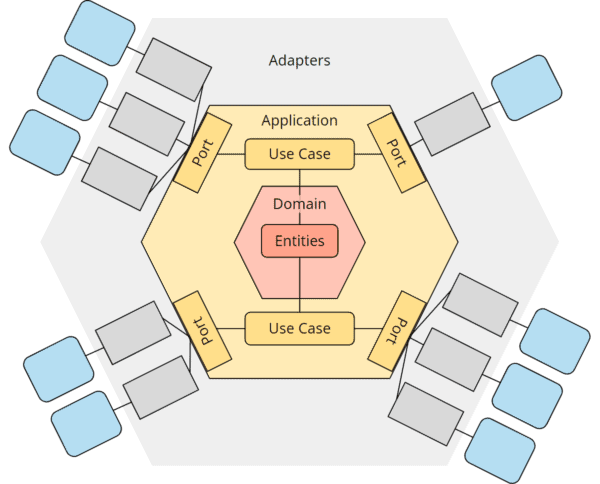
\includegraphics[width=0.5\linewidth]{image.png}
    \caption{Enter Caption}
    \label{fig:placeholder}
\end{figure}

\section{Introduction}

Designing reliable software for cyber-physical systems (e.g.\ drones, robots, autonomous vehicles) requires more than just writing code that runs. 
It requires a principled approach to structuring the software such that logic, hardware interaction, and operating system details are separated. 
This separation fosters modularity, portability, and long-term maintainability. 
In this chapter we outline a general philosophy for embedded systems architecture using a layered approach inspired by ports-and-adapters (also known as the hexagonal architecture).

\section{Motivation}

Embedded systems integrate three worlds:
\begin{enumerate}
    \item \textbf{The application logic} --- the mathematical and algorithmic core, e.g.\ control laws, estimators, and data fusion.
    \item \textbf{The hardware interface} --- the code that speaks to sensors, actuators, communication buses, and storage devices.
    \item \textbf{The middleware} --- the operating system or runtime services that schedule tasks, manage concurrency, and orchestrate communication.
\end{enumerate}

Without clear boundaries, these three concerns tend to intertwine. 
The result is fragile software that is difficult to port to new hardware or to test in isolation. 
A layered philosophy addresses this by enforcing strict separation of responsibilities.

\section{Core Logic Layer}

At the center lies the \emph{core logic layer}. 
This layer contains:
\begin{itemize}
    \item State estimation and sensor fusion algorithms.
    \item Controllers (e.g.\ PID, cascaded angle-rate loops).
    \item Mixers that translate control outputs into actuator commands.
    \item Safety mechanisms such as failsafe behaviour.
    \item Telemetry formatting and semantics.
\end{itemize}

A key design rule is that the core layer must remain \textbf{platform independent}. 
It does not include device drivers, operating system calls, or hardware registers. 
Instead, it depends only on abstract interfaces that define what the system \emph{requires} (e.g.\ ``read IMU sample'', ``write motor outputs'', ``send telemetry'').

\section{Ports and Adapters}

Between the core and the physical world sit the \emph{ports and adapters}. 
\begin{itemize}
    \item \textbf{Ports} are abstract interfaces, defined in the core, that describe required capabilities such as reading a sensor, commanding an actuator, or storing configuration data.
    \item \textbf{Adapters} are concrete implementations of these ports for a specific platform. 
          For example, one adapter may implement the motor control port using PWM timers on an ARM microcontroller, while another implements the same port using LEDC on an ESP32. 
\end{itemize}

This inversion of dependencies (the core depends only on abstractions, not concrete drivers) allows us to swap hardware, libraries, or protocols without touching the control logic.

\section{Middleware Layer}

The middleware layer encompasses the runtime environment and operating system services:
\begin{itemize}
    \item Task scheduling and priorities (e.g.\ FreeRTOS tasks at fixed update rates).
    \item Communication orchestration (e.g.\ network discovery, pairing protocols).
    \item Synchronization primitives for safe access to shared state.
\end{itemize}

The middleware injects concrete adapters into the core at startup. 
It is the \emph{composition root}, responsible for wiring together the system: instantiating drivers, providing clock sources, and starting scheduled tasks.

\section{External Entities}

Finally, beyond the software layers are the \emph{external entities}:
\begin{itemize}
    \item Physical hardware such as sensors, actuators, and microcontrollers.
    \item Human operators and controllers.
    \item Ground stations or monitoring clients.
\end{itemize}

These interact with the system exclusively through the defined adapters and ports. 
This ensures that the boundary between ``inside the software'' and ``outside in the world'' is explicit and testable.

\section{Benefits of the Layered Philosophy}

This separation yields several advantages:
\begin{enumerate}
    \item \textbf{Portability}: Core logic runs unchanged on different microcontrollers or operating systems, as long as suitable adapters exist.
    \item \textbf{Testability}: The core can be simulated on a desktop computer with mock adapters, enabling unit tests and hardware-in-the-loop simulation.
    \item \textbf{Maintainability}: Hardware upgrades or protocol changes only require replacing or extending adapters, not rewriting algorithms.
    \item \textbf{Clarity}: A well-defined architecture provides a conceptual map, reducing coupling and making reasoning about safety and performance easier.
\end{enumerate}

\section{Conclusion}

The general philosophy presented here is applicable to a wide range of embedded and control systems. 
By clearly distinguishing between the logic, the hardware interface, and the middleware, engineers can create software that is modular, reusable, and robust. 
This layered approach transforms complex projects from monolithic and brittle implementations into structured systems that can evolve over time without losing reliability.

\chapter*{ General conclusion}


% Bibliography

\printbibliography

\end{document}
